\begin{chapter}{Morse Eigenfunctions}
As a prerequisite for the ladder operators we look at the analytical solution of the Schrödinger equation with the Morse potential
as done in \cite{Landau1981Quantum}. The momentum representation and the moments of the wave function will be shortly calculated.

\section{Analytic Solution} % (fold)
\label{sec:Analytic Solution}
We denote the Morse eigenfunction by $\mu(x)$ and start with the following form of the Schrödinger equation
\begin{equation}
    \mu''(x)+\frac{2}{\varepsilon^4}( E-V_0e^{-2\beta x}+2V_0e^{-\beta x} )\mu(x)=0
\end{equation}

To solve the Schrödinger equation for the Morse potential we first have to transform the  position variable $x$ to get rid of the exponentials:
\begin{equation}
    \label{eq:morse_var_transform}
    z:=\nu e^{-\beta x},\qquad \nu=\sqrt{\frac{8V_0}{\beta^2\varepsilon^4}}
\end{equation}

Furthermore, to simplify notation we introduce an additional constant $s(n,\nu)$, which, using the quantum number $n$, can be written as
\begin{equation}
    \label{eq:const_rel}
    s:=-n+\frac{1}{2}\nu-\frac{1}{2}\; .
\end{equation}

\subsection{Variable Transformation}
Applying the transformation and substituting the new constants yields
\begin{align}
    &\mu''(z)\nu^2\beta^2e^{-2\beta x}+\mu'(z)\nu\beta^2e^{-\beta x}+\frac{2m}{\hbar^2}\left(E-V_0\frac{z^2}{\nu^2}+2V_0\frac{z}{\nu}\right)\mu(z)\\
    &=\mu''(z)z^2+\mu'(z)z+\left[\frac{2m}{\hbar^2\beta^2}E-\underbrace{\frac{2mV_0}{\hbar^2\beta^2}}_{1/4 \nu^2}\frac{z^2}{\nu^2}
	+\underbrace{\frac{4mV_0}{\hbar^2\beta^2}}_{1/2\nu^2}\frac{z}{\nu}\right]\mu(z)\\
    &=\mu''(z)+\frac{\mu'(z)}{z}-\left[\frac{s^2}{z^2}+\frac{1}{4}-\frac{1}{z}\underbrace{\frac{1}{2}\nu}_{n+s+\frac{1}{2}} \right]
    \mu(z)\;,
\end{align}
such that we arrive at the following simplified equation:
\begin{equation}
	\label{eq:morse_transformed_tdse}
	\mu''(z)+\frac{\mu'(z)}{z}+\left( -\frac{1}{4}+\frac{n+s+\frac{1}{2}}{z}-\frac{s^2}{z^2}\right)\mu=0
\end{equation}


\subsection{Asymptotic Solutions}
For solving \eqref{eq:morse_transformed_tdse} we investigate the asymptotics of this equation. For $z\to\infty$ 
\eqref{eq:morse_transformed_tdse} becomes 
\begin{equation}
   \mu_a''(z)=\frac{1}{4}\mu_a(z)
\end{equation}
which is solved by
\begin{equation}
    \mu_a=e^{\pm\frac{1}{2}z}
\end{equation}
and we must chose $\frac{1}{2}$ to obtain a normalizable wave function.\\
Similarly  for $z\to 0$ we have
\begin{equation}
 \mu_a''(z)=\frac{s^2}{z^2}\mu_a(z) 
\end{equation}
solved by
\begin{equation}
    \mu_a(z)=z^{\pm s}
\end{equation}
and we must choose $+s$ to avoid divergence at $z=0$.\\

To account for this asymptotic behavior, we consequently choose the following ansatz:
\begin{equation}
	\label{eq:asymp_ansatz}
	\mu(z)=e^{-\frac{z}{2}}z^{s}w(z)
\end{equation}

After plugging \eqref{eq:asymp_ansatz} into \eqref{eq:morse_transformed_tdse} we obtain the much simpler differential equation
\begin{equation}
	zw''+(2s+1-z)w'+nw=0
\end{equation}
which is solved by the \textit{confluent hypergeometric function} $\mathrm{F}$:
\begin{equation}
    w(z)= {}_{1}F_1(-n;2s+1;z)=L_n^{2s}(z)
\end{equation}
For the special case of $n\in\mathbbm{N}$ this becomes the generalized Laguerre polynomials $\mathrm{L}_{n}^{2s}$
such that we finally arrive at the full solution
\begin{equation}
    \label{eq:morse_function}
  \mu_{n}(z) = N_{n} e^{-\frac{z}{2}} z^{s} \mathrm{L}_{n}^{2s}(z).
\end{equation}
where $s := \frac{\nu - 2n -1}{2}$. The normalization constant $N_n$ will be determined in the next section.\\
Plots of the first few Morse states can be seen in Figures \ref{fig:MorseRe0_2} and \ref{fig:MorseRe0_11}.


\begin{figure}[h!]
	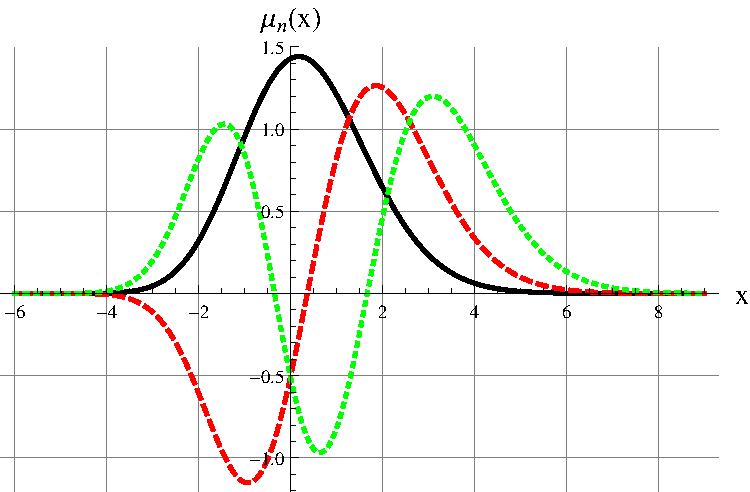
\includegraphics[width=1.0\linewidth]{./figures/MorseWavefunctions/MorseRe0_2.pdf}
       \caption[Morse Wavefunction for $n=0,1,2$]{
	   Plot of the real parts (imaginary part is zero) of the first three Morse eigenstates.
	   (n=0 (solid, black), n=1 (dashed, red), n=2 (dotted, green))\\
	   The parameters $V_0=4.$ and $\beta=0.2$ were chosen.
	\label{fig:MorseRe0_2}
    }

\end{figure}


\begin{figure}[h!]
	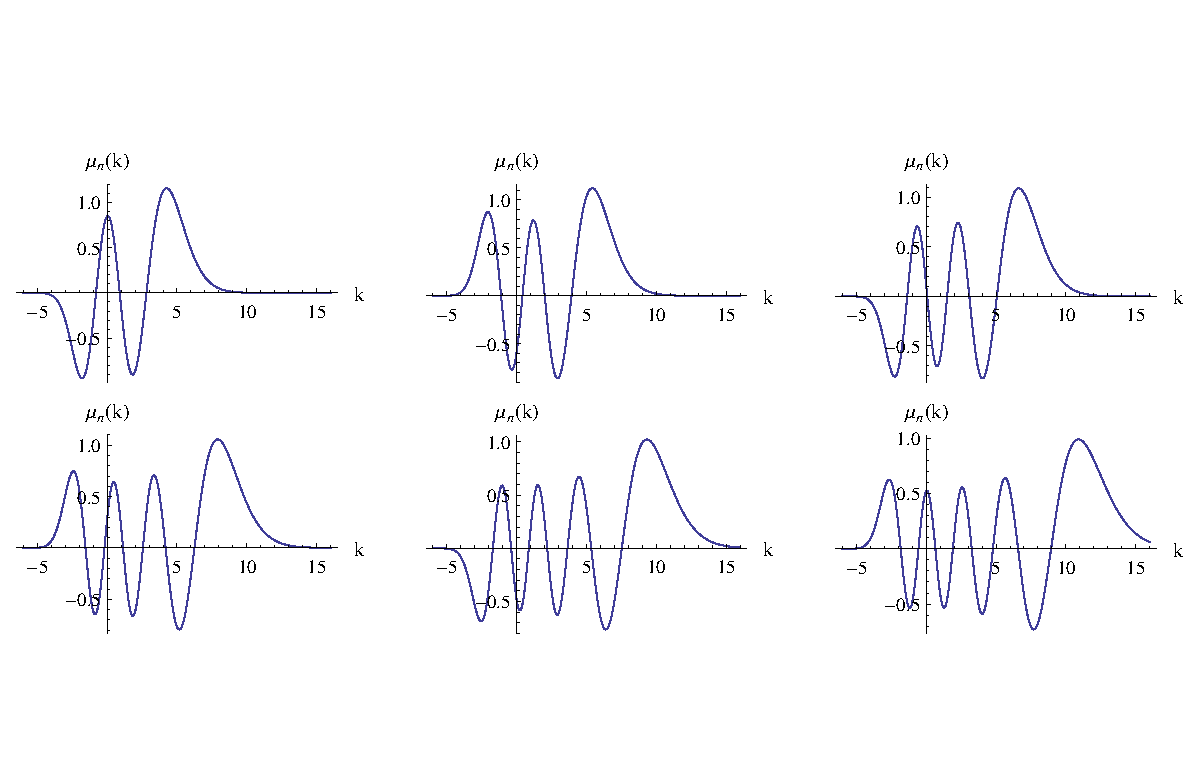
\includegraphics[width=1.0\linewidth]{./figures/MorseWavefunctions/MorseRe0_11.pdf}
       \caption[Morse Wavefunction for $n=3,\ldots,8$]{
	   Higher states of the Morse potential, quantum number $n=3,\ldots,8$ increases from left to right and top to bottom.
	   The parameters $V_0=4.$ and $\beta=0.2$ were chosen.
	\label{fig:MorseRe0_11}
    }

\end{figure}



\subsection{Normalization} % (fold)
\label{sub:Normalization}

In order to calculate the normalization constant $N_n$ we have to compute the following integral
\footnote{Since $\mu_n(z)\in\mathbbm{R}$ we will omit complex conjugation from now on}:
\begin{equation}
  \langle \mu_{m}(x) | \mu_{n}(x) \rangle = \int_{-\infty}^{\infty} \overline{\mu_{m}(x)} \mu_{n}(x) \mathrm{d}x \,.
\end{equation}

Based on the variable transformation \eqref{eq:morse_var_transform} the differential transforms as
\begin{equation}
  \mathrm{d}x = -\frac{1}{\beta z} \mathrm{d}z \,.
\end{equation}
while for the integration boundaries we have
\begin{equation}
  \begin{split}
    z(x) = \infty & \quad x \rightarrow -\infty \\
    z(x) = 0 & \quad x \rightarrow \infty  \,.
  \end{split}
\end{equation}
such that we arrive at the overlap integral
\begin{equation}
  \label{eq:overlap}
  \begin{split}
    \int_{-\infty}^{\infty} \mu_{m}(x) \mu_{n}(x) \mathrm{d}x
    & = - \int_{\infty}^{0} \mu_{m}(z) \mu_{n}(z) \frac{1}{\beta z} \mathrm{d}z \\
    & = \frac{1}{\beta} \int_{0}^{\infty} \mu_{m}(z) \mu_{n}(z) \frac{1}{z} \mathrm{d}z \\
    & =: \frac{1}{\beta} I \,.
  \end{split}
\end{equation}

$I$ can be explicitly written as:
\begin{equation}
  \begin{split}
    I
    & = \int_{0}^{\infty} N_{n} e^{-\frac{z}{2}} z^{s} \mathrm{L}_{n}^{2s}(z) N_{n} e^{-\frac{z}{2}} z^{s} \mathrm{L}_{n}^{2s}(z) \frac{1}{z} \mathrm{d}z \\
    & = N_{n}^{2} \int_{0}^{\infty} e^{-z} z^{2s} \mathrm{L}_{n}^{2s}(z)^{2} \frac{1}{z} \mathrm{d}z \\
    & = N_{n}^{2} \int_{0}^{\infty} e^{-z} z^{\alpha - 1} \mathrm{L}_{n}^{\alpha}(z)^{2} \mathrm{d}z
  \end{split}
\end{equation}
where $\alpha := 2s$. We use the following formula
\footnote{\url{http://functions.wolfram.com/Polynomials/LaguerreL3/21/02/01/0003/}}:
\begin{equation}
  \begin{split}
    I
    & = \int_{0}^{\infty} t^{\alpha - 1} e^{-\lambda t} \mathrm{L}_{m}^{\alpha_{m}}(\lambda t) \mathrm{L}_{n}^{\alpha_{n}}(\lambda t) \mathrm{d}t \\
    & = \frac{\lambda^{-\alpha} \Gamma(\alpha) \Gamma(n-\alpha+\alpha_{n}+1) \Gamma(m+\alpha_{m}+1)}
             {m! n! \Gamma(1-\alpha+\alpha_{n}) \Gamma(\alpha_{m}+1)}
        {}_{3}F_{2}
        \left(
          \begin{matrix}
            - m, \alpha, \alpha - \alpha_{n} \\
            \alpha - \alpha_{n} - n, \alpha_{m} + 1
          \end{matrix}
          \middle| {1} \right) \,.
  \end{split}
\end{equation}

In our case $\lambda = 1$ and for $m = n$ we also have $\alpha_{m} = \alpha_{n}$:
\begin{equation}
  I = \frac{\Gamma(\alpha) \Gamma(n+\alpha_{n}+1) \Gamma(n-\alpha+\alpha_{n}+1)}
           {(n!)^{2} \Gamma(\alpha_{n}+1) \Gamma(\alpha_{n}-\alpha+1)}
      {}_{3}F_{2}
      \left(
        \begin{matrix}
          -n, \alpha, \alpha-\alpha_{n} \\
          -n+\alpha -\alpha_{n}, \alpha_{n}+1
        \end{matrix}
      \middle| {1} \right) \,.
\end{equation}
Defining $\alpha_{n} = \alpha$ yields:
\begin{equation}
  I = \frac{\Gamma(n+\alpha+1)}{\alpha \Gamma(n+1)}
\end{equation}
and using the relation $\alpha := \nu - 2n - 1$:
\begin{equation}
  \label{eq:norm_integral}
  I = \frac{\Gamma(\nu-n)}{(\nu -2n -1) \Gamma(n+1)}
\end{equation}
such that we finally arrive at our normalization constant
\begin{equation}
  N_{n} = \sqrt{\beta \frac{(\nu -2n -1) \Gamma(n+1)}{\Gamma(\nu-n)}} \,.
\end{equation}
% subsection Normalization (end)

\subsection{Orthonormality}

Now starting again from \eqref{eq:overlap} we need to explicitly compute
\begin{equation}
  \begin{split}
    J
    & = \int_{0}^{\infty} N_{m} e^{-\frac{z}{2}} z^{s_{m}} \mathrm{L}_{m}^{2s_{m}}(z)
                          N_{n} e^{-\frac{z}{2}} z^{s_{n}} \mathrm{L}_{n}^{2s_{n}}(z)
                          \frac{1}{z} \mathrm{d}z \\
    & = N_{m} N_{n} \int_{0}^{\infty} e^{-z} z^{s_{m}+s_{n}}
					  \mathrm{L}_{m}^{2s_{m}}(z)
					  \mathrm{L}_{n}^{2s_{n}}(z)
					  \frac{1}{z} \mathrm{d}z \\
	& = N_{m} N_{n} \int_{0}^{\infty} e^{-z} z^{\frac{\alpha_{m}+\alpha_{n}}{2}-1}
					  \mathrm{L}_{m}^{\alpha_{m}}(z)
					  \mathrm{L}_{n}^{\alpha_{n}}(z)
					  \mathrm{d}z
      \end{split}
    \end{equation}
    where $\alpha_{m} := 2s_{m}$ and $\alpha_{n} := 2s_{n}$.
    To solve this integral we use the formula
    \footnote{ \url{http://functions.wolfram.com/Polynomials/LaguerreL3/21/02/01/0002/}}:
    \begin{equation*}
      \begin{split}
	J
	& = \int_{0}^{\infty} t^{\alpha-1} e^{-\lambda t} \mathrm{L}_{m}^{\alpha_{m}}(a_{m} t) \mathrm{L}_{n}^{\alpha_{n}}(a_{n} t) \mathrm{d}t \\
	& = \frac{\lambda^{-\alpha}\Gamma(\alpha) \left(\alpha_{m}+1\right)_{m} \left(\alpha_{n}+1\right)_{n}}{m! n!}
	\sum_{j=0}^{m} \frac{(-m)_{j} (\alpha)_{j}}{\left(\alpha_{m}+1\right)_{j} j!} \left(\frac{a_{m}}{\lambda}\right)^{j}
	\sum_{k=0}^{n} \frac{(-n)_{k} (\alpha+j)_{k}}{\left(\alpha_{n}+1\right)_{k} k!} \left(\frac{a_{n}}{\lambda}\right)^{k} \,.
      \end{split}
    \end{equation*}
    where $a_{m} = 1$, $a_{n} = 1$ and $\lambda = 1$:
    \begin{equation*}
      \begin{split}
	J
	& = \frac{\Gamma(\alpha) \left(\alpha_{m}+1\right)_{m} \left(\alpha_{n}+1\right)_{n}}{m! n!}
	\sum_{j=0}^{m} \frac{(-m)_{j} (\alpha)_{j}}{\left(\alpha_{m}+1\right)_{j} j!}
	\sum_{k=0}^{n} \frac{(-n)_{k} (\alpha+j)_{k}}{\left(\alpha_{n}+1\right)_{k} k!} \\
	& =
	\frac{\alpha_{n}! \Gamma(\alpha) \left(\alpha_{m}+1\right)_{m} \left(\alpha_{n}+1\right)_{n} (\alpha_{n}+\alpha+n)!}
	     {m! n! (\alpha_n-\alpha)! (\alpha_n+n)!}
	{}_{3}F_{2}
	\left(
	  \begin{matrix}
	    -m, \alpha, \alpha-\alpha_{n} \\
	    \alpha_{m}+1, \alpha-\alpha_{n}-n
	  \end{matrix}
	  \middle| {1} \right) \,.
      \end{split}
    \end{equation*}
    Furthermore, inserting $\alpha = \frac{\alpha_{m} + \alpha_{n}}{2}$,
    $\alpha_{m} = \nu - 2m -1$ and $\alpha_{n} = \nu -2n -1$ yields
    \begin{equation}
      J = \frac{\Gamma(\nu-m)}{(\nu-m-n-1) \Gamma(n+1) \Gamma(1+m-n) \Gamma(1-m+n)}
    \end{equation}
    In the case $m = n$ we arrive at \eqref{eq:norm_integral} again.
    Otherwise, using the Euler formula
    \footnote{
      \begin{equation}
	\Gamma(1 + z) \Gamma(1 - z) = \frac{\pi z}{\sin(z \pi)}
      \end{equation}
    }
    the result can be simplified to
    \begin{equation}
      J = \frac{\Gamma(\nu-m)}{(\nu-m-n-1) \Gamma(n+1)}\frac{\sin((m-n)\pi)}{\pi (m-n)}
    \end{equation}
    Now, since  $\sin((m-n)\pi) = 0$ for $m, n \in \mathbb{N}$ it follows, that
    \begin{equation}
      J = 0
    \end{equation}

    % section Analytic Solution (end)

    \section{Momentum Representation} % (fold)
    \label{sec: Momentum Representation}
    Our motivation for calculating the Fourier transformation of the Morse states is the observation in \cite{H_ladder_operators} that in the case of Hagedorn wave packets 
    the variables $(x, q)$ and $(y,p)$, as well as the parameters $Q$ and $P$, up to a sign and a global phase factor simply switch roles in the
    formulas after transformation to momentum space:

\begin{equation}
    \label{eq:HGWavepacketFourier}
    (\mathcal{F}\phi_k(Q, P, \hbar, q, p, x))(y)=(-i)^ke^{-ia\eta/\hbar}\phi_k(Q, P, \hbar, \eta, -q, y)
\end{equation}

Although it might be that this is solely due to the fact that the Gaussians are eigenfunctions of the Fourier transformation it is nevertheless useful to check
if there is any obvious symmetry recognizable in the Morse case after transformation.\\
Apart from that the results might also be useful to compute certain matrix elements in future applications.\\

We recall that the  Morse wave packet $\mu_{n}$ is given by:

\begin{equation}
  \mu_{n}(z) = N_{n} e^{-\frac{z}{2}} z^{s} L_{n}^{2s}(z)
\end{equation}

and with $z = \nu \exp(-\beta x)$ we have:

\begin{equation}
  \mu_{n}(x) = N_{n} e^{-\frac{\nu}{2} \exp(-\beta x)} \nu^{s} \exp(-\beta x)^{s} L_{n}^{2s}\left(\nu \exp(-\beta x)\right)
\end{equation}

\subsection{Ground State}
Since for $n=0$ the Laguerre polynomials equal unity, we first try to compute the Fourier transformation of the ground state $\mu_{0}$:

\begin{equation}
  \mu_{0}(x) = N_{0} e^{-\frac{\nu}{2} \exp(-\beta x)} \nu^{s} \exp(-\beta x)^{s} \underbrace{L_{n}^{2s}\left(\nu \exp(-\beta x)\right)}_{\equiv 1}
\end{equation}

which is proportional to the following kernel:

\begin{equation}
  \mu_{0}(x) \sim e^{-\alpha e^{-\beta x}} \left(e^{-\beta x}\right)^{\gamma}
\end{equation}

where $\alpha = \frac{\nu}{2}$ and $\gamma = s$. Next we try to compute its
Fourier transformation:

\begin{align}
  \ft{e^{-\alpha e^{-\beta x}} \left(e^{-\beta x}\right)^{\gamma}}(k)
  & = \frac{1}{\sqrt{2\pi}} \int_{-\infty}^{\infty} e^{-\alpha e^{-\beta x}} \left(e^{-\beta x}\right)^{\gamma} e^{- i k x} \di{x} \\
  & = \frac{1}{\sqrt{2\pi}}
  \frac{1}{\beta}
  \alpha^{-\gamma -\frac{i k}{\beta}}
  \Gamma \left(\gamma+\frac{i k}{\beta}\right) \,.
\end{align}

Finally we get the transformation of the wave packet $\mu_{0}$:

\begin{equation*}
  \hat{\mu_{0}}(k) = \ft{\mu_{0}(x)} =
  \frac{N_{0}}{\sqrt{2\pi}}
  \frac{\nu^{s}}{\beta}
  \left(\frac{\nu}{2}\right)^{-s -\frac{i k}{\beta}}
  \Gamma \left(s+\frac{i k}{\beta}\right)
\end{equation*}

\subsection{Higher States}

Next we look at the higher order states $n>0$. This time we need to include
the Laguerre polynomial $L_{n}^{a}(x)$. In order to so we choose the following representation of the Laguerre polynomials:

\begin{equation}
  L_{n}^{a}(z) := \sum_{i=0}^{n} \frac{(-1)^{i}}{i!}
                                \frac{\Gamma(n+a+1)}{\Gamma(a+1+i) \Gamma(n+1-i)}
                                z^{i}
                = \sum_{i=0}^{n} C_{n,a,i} \, z^{i} \,.
\end{equation}

Applying again the coordinate transformation we find that:

\begin{equation}
  L_{n}^{2s}(z)
  = L_{n}^{2s}\left(\nu \exp(-\beta x)\right)
  = \sum_{i=0}^{n} C_{n,2s,i} \, \left(\nu \exp(-\beta x)\right)^{i}
\end{equation}

and since $i$ is a nonnegative integer we have:

\begin{equation}
  L_{n}^{2s}(x) = \sum_{i=0}^{n} C_{n,2s,i} \, \nu^{i} \exp(- i \beta x) \,.
\end{equation}

The higher order states $\mu_{n}(x)$ can therefore be written like:

\begin{align}
  \mu_{n}(x)
  & = N_{n} e^{-\frac{\nu}{2} \exp(-\beta x)} \nu^{s} \exp(-\beta x)^{s} \sum_{i=0}^{n} C_{n,2s,i} \, \nu^{i} \exp(- i \beta x) \\
  & = \sum_{i=0}^{n} N_{n} C_{n,2s,i} \, \nu^{s+i} e^{-\frac{\nu}{2} \exp(-\beta x)} \exp(-\beta x)^{s} \exp(- i \beta x) \,.
\end{align}

We can compute the Fourier transformation of a slightly extended kernel:

\begin{align}
  \ft{e^{-\alpha e^{-\beta x}} \left(e^{-\beta x}\right)^{\gamma} e^{- i \beta x}}(k)
  & = \frac{1}{\sqrt{2\pi}}
  \frac{1}{\beta}
  \alpha^{-\gamma -i -\frac{i k}{\beta}}
  \Gamma \left(\gamma+i+\frac{i k}{\beta}\right) \,.
\end{align}

For the wave packet we in turn find:

\begin{equation}
  \hat{\mu_{n}}(k) = \ft{\mu_{n}(x)} =
  \sum_{i=0}^{n}
  N_{n} C_{n,2s,i} \, \nu^{s+i}
  \frac{1}{\sqrt{2\pi}}
  \frac{1}{\beta}
  \left(\frac{\nu}{2}\right)^{-s -i -\frac{i k}{\beta}}
  \Gamma \left(s+i+\frac{i k}{\beta}\right)
\end{equation}

where the constant is $C_{n,2s,i} = \frac{(-1)^{i}}{i!} \frac{\Gamma(n+2s+1)}{\Gamma(2s+1+i) \Gamma(n+1-i)}$. It is indeed possible to resolve this sum and obtain a relatively simple formula:

\begin{equation*}
  \hat{\mu}_{n}(k) =
  \frac{N_{n}}{\sqrt{2\pi}}
  \frac{2^{s+\frac{i k}{\beta}} \nu^{-\frac{i k}{\beta}}}{\beta}
  \frac{\Gamma(1+n+2s)}{\Gamma(1+n)\Gamma(1+2s)}
  \Gamma\left(s+\frac{i k}{\beta}\right)
  {}_{2}F_{1}
  \left(
    \begin{matrix}
      - n, s + \frac{i k}{\beta} \\
      2s + 1
    \end{matrix}
    \middle| {2} \right)
\end{equation*}

Again we provide some plots of the Morse states in the Figures

\begin{figure}[h!]
	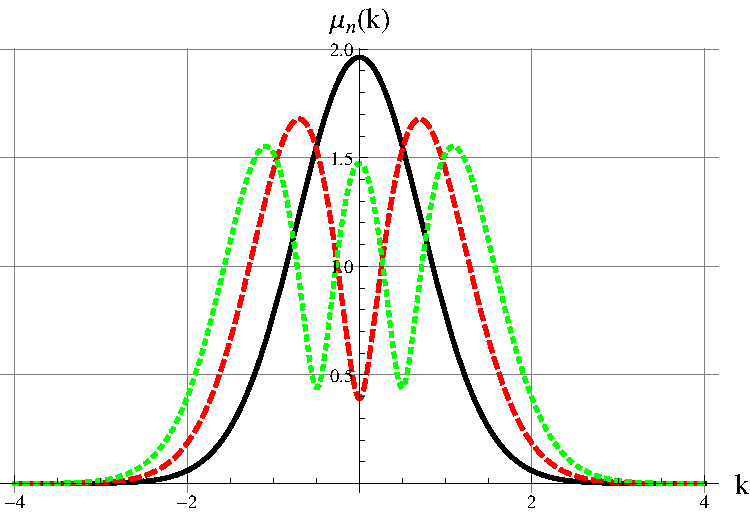
\includegraphics[width=1.0\linewidth]{./figures/MorseFourier/FourierAbsn0_2.pdf}
       \caption[Morse momentum wavefunction for $n=0,1,2$]{
	   Plot of the absolute modulus of the first three Morse eigenstates in momemtum space
	   (n=0 (solid, black), n=1 (dashed, red), n=2 (dotted, green))\\
	   The parameters $V_0=4.$ and $\beta=0.2$ were chosen.
	\label{fig:FourierAbsn0_2}
    }

\end{figure}


\begin{figure}[h!]
	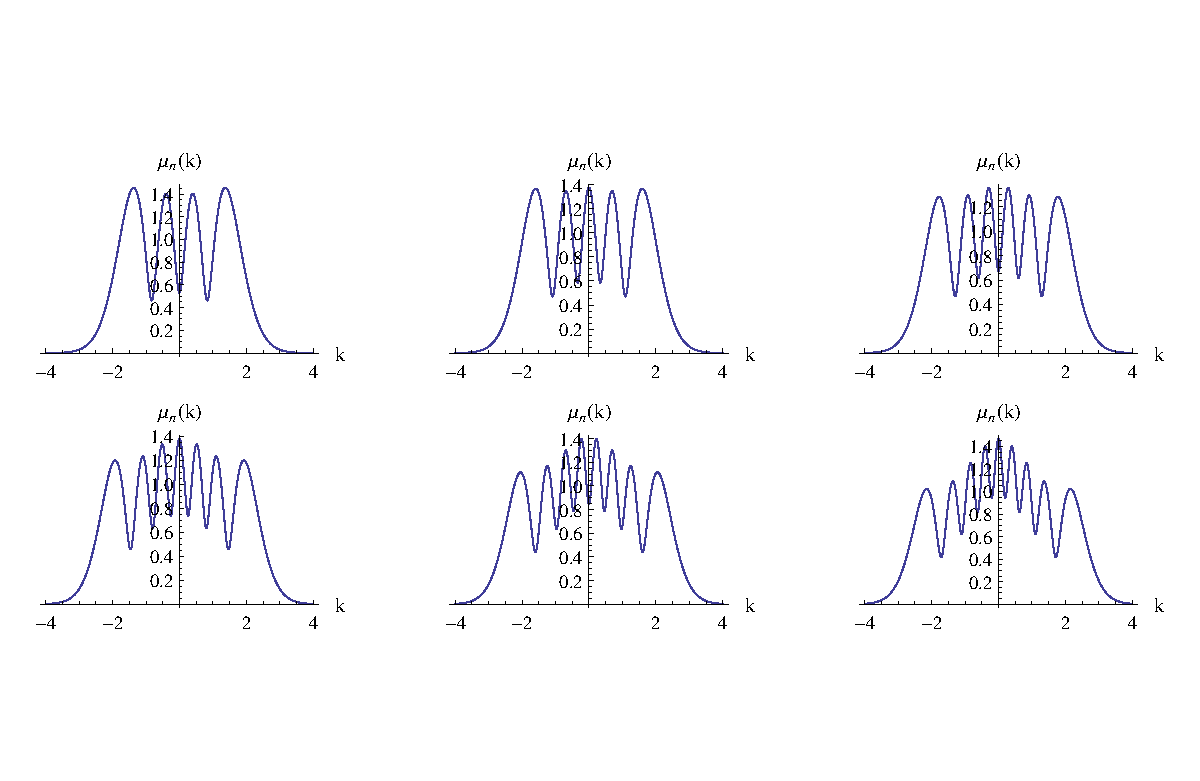
\includegraphics[width=1.0\linewidth]{./figures/MorseFourier/FourierAbsn0_11.pdf}
       \caption[Morse momentum wavefunction for $n=3,\ldots,8$]{
	   Higher states of the Morse potential in momentum space, quantum number $n=3,\ldots,8$ increases from left to right and top to bottom.
	   The parameters $V_0=4.$ and $\beta=0.2$ were chosen.
	\label{fig:FourierAbsn0_11}
    }

\end{figure}


% section Momentum Representation (end)

\section{Moments} % (fold)
\label{sec:Moments}
As explained in the introduction, the parameters $Q$ and $P$ can be interpreted as the width in position and momentum space, respectively.
Since the probability distribution $|\mu_n|^2$ describes the localization of the particle, calculating its first two central moments 
provides us with analytical expressions for the mean position and standard deviation. This might again give hints about the parameters.
In addition to that we also calculate some important diagonal matrix elements for the Morse function which we will then, using the ladder operator
formalism introduced in the next section, generalize to other operators.\\

We start again with the following expression
\begin{equation}
  \mu_{n}(x) = N_{n} e^{-\frac{\nu}{2} \exp(-\beta x)} \nu^{s} \exp(-\beta x)^{s} L_{n}^{2s}\left(\nu \exp(-\beta x)\right)\;.
\end{equation}


The following properties about the various parameters hold:
\begin{align}
  & n \in \mathbb{N} \\
  & \beta \in \mathbb{R}, \beta > 0 \\
  & V_{0} \in \mathbb{R}, V_{0} > 0 \\
  & N_{n} \in \mathbb{R} \,,
\end{align}

from the condition $\nu - 2n - 1 =: w > 0$ and $s := \frac{w}{2}$ we find that:

\begin{align}
  & \nu \in \mathbb{R}, \nu > 0 \\
  & s \in \mathbb{R}, s > 0 \,.
\end{align}

\subsection{First moment of the ground state}

The task is to compute the first moment:

\begin{equation}
  \braket{\mu_{0} | x | \mu_{0}} = \int_{-\infty}^{\infty} \mu_{0}(x) x \mu_{0}(x) \di{x} \,.
\end{equation}

With:

\begin{equation}
  \mu_{0}(x) = N_{0} \underbrace{e^{-\frac{\nu}{2} e^{-\beta x}}}_{A(x)} \nu^{s} \underbrace{\left(e^{-\beta x}\right)^{s}}_{B(x)}
\end{equation}

we find:

\begin{align}
    \int_{-\infty}^{\infty} \mu_{0(x)} x \mu_{0}(x) \di{x}
  & =   \int_{-\infty}^{\infty} N_{0} \nu^{s} A(x) B(x) x N_{0} \nu^{s} A(x) B(x) \di{x} \\
  & =   N_{0}^{2} \nu^{2s} \int_{-\infty}^{\infty} A(x) B(x) x A(x) B(x) \di{x} \\
  & =   N_{0}^{2} \nu^{2s} \int_{-\infty}^{\infty} A(x)^{2} B(x)^{2} x \di{x} \,.
\end{align}

The last equality holds since $A(x)$ and $B(x)$ are real valued.
This integral can be written in general form like shown in \eqref{int:def_1}
and substitution of $\alpha=\nu$ and $\gamma=2s$ gives for the first moment:

\begin{equation}
    \braket{\mu_{0} | x | \mu_{0}}
    = \frac{N_{0}^{2}}{\beta^{2}} \Gamma(\nu-1) \left(\log(\nu) - \psi^{(0)}(\nu-1)\right)
\end{equation}
where for $n=0$ we have by definition $2s = \nu - 1$ and $\psi^{(i)}$ denotes the polygamma function of
order $i$ defined as the $i+1$-th derivative of the logarithm of the gamma function:
\begin{align}
\psi^{(i)}(z)=\pdiff{^{m+1}}{z^{m+1}}\log \Gamma(z)
\end{align}



\subsection{Second moment of the ground state}


For the second central moment we have:

\begin{equation}
  \braket{\mu_{0} | (x-q)^{2} | \mu_{0}}
  = \braket{\mu_{0} | x^{2} | \mu_{0}}
  - 2 q \braket{\mu_{0} | x | \mu_{0}}
  + q^{2} \braket{\mu_{0} | \mu_{0}}
\end{equation}

hence we first compute:

\begin{align}
  \braket{\mu_{0} | x^{2} | \mu_{0}}
  & = \int_{-\infty}^{\infty} \conj{\mu_{0(x)}} x^{2} \mu_{0}(x) \di{x} \\
  & =   N_{0}^{2} \nu^{2s} \int_{-\infty}^{\infty} A(x)^{2} B(x)^{2} x^{2} \di{x} \,.
\end{align}

The basic integral we need here is given in \eqref{int:def_2} and
applying the same substitution of $\alpha=\nu$ and $\gamma=2s$ again
 gives the second moment:

\begin{align}
    \braket{\mu_{0} | x^{2} | \mu_{0}}
    = \frac{N_{0}^{2}}{\beta^{3}} \Gamma(\nu-1) \left(\left(\log(\nu) - \psi^{(0)}(\nu-1) \right)^{2} + \psi^{(1)}(\nu-1) \right)
\end{align}


\subsection{Moments of higher states}


The aim of this section is the computation of $k$-th moments for higher states $\mu_{n}$.
This is not straight-forward but can be done step by step. We start with:

\begin{align}
  \label{eq:def_kth_mom}
  \braket{\mu_{n} | x^{k} | \mu_{n}}
  & = \int_{-\infty}^{\infty} \conj{\mu_{n}(x)} x^{k} \mu_{n}(x) \di{x} \\
  & = \int_{-\infty}^{\infty} \conj{N_{n} \nu^{s} A(x) B(x) L_{n}^{2s}(\delta)}
                                \, x^{k} \,
                                N_{n} \nu^{s} A(x) B(x) L_{n}^{2s}(\delta) \,\di{x} \\
  & =   N_{n}^{2} \nu^{2s} \int_{-\infty}^{\infty} A(x)^{2} B(x)^{2} \left( L_{n}^{2s}(\delta) \right)^{2} x^{k} \,\di{x}
\end{align}

where $\delta := \nu \exp(-\beta x)$. Before we can continue we need an explicit expansion
for the square of Laguerre polynomials. This is a classical result by W. N. Bailey
and W. T. Howell\footnote{
We use the following definition of Laguerre polynomials:
\begin{equation*}
  L_{n}^{a}(z)
  :=
  \frac{\Gamma(n+a+1)}{\Gamma(n+1) \Gamma(a+1)}
  \,
  {}_{1}F_{1}
  \left(
    \begin{matrix}
      - n \\
      a+1
    \end{matrix}
    \middle| {x} \right)
\end{equation*}
and have to divide by an additional factor $\Gamma(a+1)$ compared to the original paper.}:

\begin{align}
  \left( L_{n}^{a}(z) \right)^{2}
  & =
  \underbrace{\frac{\Gamma(1+n+a)}{\Gamma(1+a) 2^{2n}n!}}_{=: G_{n,a}}
  \sum_{r=0}^{n}
  \underbrace{\frac{(2r)! (2n-2r)!}{\Gamma(1+r) \Gamma(1+n-r)^{2} \Gamma(1+r+a)}}_{=: F_{n,a,r}}
  L_{2r}^{2a}(2z) \\
  & =
  G_{n,a} \sum_{r=0}^{n} F_{n,a,r} L_{2r}^{2a}(2z) \,.
\end{align}

Combining this with the explicit expression for the Laguerre polynomials:

\begin{equation}
  L_{n}^{a}(z)
  :=
  \sum_{i=0}^{n}
  \underbrace{
    \frac{(-1)^{i}}{i!}
    \frac{\Gamma(n+a+1)}{\Gamma(a+1+i) \Gamma(n+1-i)}
  }_{=: C_{n,a,i}}
  z^{i}
  = \sum_{i=0}^{n} C_{n,a,i} \, z^{i} \,.
\end{equation}

we find:

\begin{equation}
  \left( L_{n}^{a}(z) \right)^{2} =
  G_{n,a}
  \sum_{r=0}^{n}
  F_{n,a,r} \,
  \sum_{i=0}^{2 r}
  C_{2r,2a,i} \, (2 z)^{i} \,.
\end{equation}

Plugging this into the integral \eqref{eq:def_kth_mom} from above yields:

\begin{align*}
  \braket{\mu_{n} | x^{k} | \mu_{n}}
  & =
  N_{n}^{2} \nu^{2s} \int_{-\infty}^{\infty} A(x)^{2} B(x)^{2}
  G_{n,2s} \sum_{r=0}^{n} F_{n,2s,r} \sum_{i=0}^{2 r} C_{2r,4s,i} \, (2 \delta)^{i} x^{k} \di{x} \\
  & =
  N_{n}^{2} \nu^{2s} G_{n,2s} \sum_{r=0}^{n} \sum_{i=0}^{2 r} F_{n,2s,r} \, C_{2r,4s,i} \, 2^{i}
  \int_{-\infty}^{\infty} A(x)^{2} B(x)^{2} \delta^{i} x^{k} \di{x} \\
  & =
  N_{n}^{2} \nu^{2s} G_{n,2s} \sum_{r=0}^{n} \sum_{i=0}^{2 r} F_{n,2s,r} \, C_{2r,4s,i} \,
  2^{i} \nu^{i}
  \int_{-\infty}^{\infty} A(x)^{2} B(x)^{2} \left(e^{-\beta x}\right)^{i} x^{k} \di{x}
\end{align*}

For the remaining integrals we use the general formula given in
\eqref{int:def_n} with the values $\alpha = \nu$ and $\gamma = 2s + i$.

\begin{align}
    \braket{\mu_{n} | x^{k} | \mu_{n}}
    =
    N_{n}^{2} \nu^{2s} G_{n,2s}
    \sum_{r=0}^{n}
    \sum_{i=0}^{2 r}
    F_{n,2s,r} \, C_{2r,4s,i} 2^{i} \nu^{i} I_{\nu,\beta,2s+i}^{(k)} \,.
\end{align}

Next we try to combine the individual parameter terms and resolve the sums.
However, it seems that this is not possible and there exists no closed form
for this nested sum.

% section Moments (end)

\end{chapter}
